% This is part of Un soupçon de mathématique sans être agressif pour autant
% Copyright (c) 2015
%   Laurent Claessens
% See the file fdl-1.3.txt for copying conditions.

% This is part of Un soupçon de mathématique sans être agressif pour autant
% Copyright (c) 2015
%   Laurent Claessens
% See the file fdl-1.3.txt for copying conditions.

%--------------------------------------------------------------------------------------------------------------------------- 
\subsection*{Activité : pliage}
%---------------------------------------------------------------------------------------------------------------------------

\begin{enumerate}
    \item
        
Prendre une feuille de papier et réaliser des pliages suivant les lignes indiquées :

    \begin{center}
        \input{Fig_DWHNooSCJJNE.pstricks}                                          
    \end{center}  

    \item

        Refermer le tout en faisant coïncider les deux bords en gras. On obtient ainsi un solide sans «fond» ni «couvercle».

    \item

        Comment s'appelle le polygone formant les bases ?

    \item

         Combien de faces comporte le solide (y compris les bases) ?
    \item
          Quelles sont les formes des autres faces appelées « faces latérales » ?
    \item
           Combien de sommets comporte ton solide ?

\end{enumerate}

De \cite{NRHooXFvgpp5}

%+++++++++++++++++++++++++++++++++++++++++++++++++++++++++++++++++++++++++++++++++++++++++++++++++++++++++++++++++++++++++++ 
\section{Prisme}
%+++++++++++++++++++++++++++++++++++++++++++++++++++++++++++++++++++++++++++++++++++++++++++++++++++++++++++++++++++++++++++

\begin{definition}
    Un \defe{prisme droit}{prisme droit} est un solide composé de deux bases qui sont superposables et parallèles et de faces latérales qui sont des rectangles.
\end{definition}


\begin{example}
    Dessiner un patron d'un prisme droit dont la base est un triangle de côtés \SI{5}{\centi\meter}, \SI{4}{\centi\meter} et \SI{3}{\centi\meter}, et dont la hauteur est égale à \SI{2}{\centi\meter} (aide : la base est un triangle rectangle).

    \begin{enumerate}
        \item
            D'abord tracer une base :


\begin{center}
   \input{Fig_JYAKooXjBUptooZERO.pstricks}
\end{center}
\item
    Ensuite les faces latérales sont des rectangles perpendiculaires à la base
\begin{center}
   \input{Fig_JYAKooXjBUptooONE.pstricks}
\end{center}
\item
    Et enfin on trace la seconde base (le «couvercle»). Le plus simple est de l'accrocher à une des faces latérales.

    Si on veut l'attacher au segment \( [FG]\), alors le côté du couvercle passant par \( F\) devra s'attacher à \( [DE]\). Il doit donc en avoir la longueur; il faut donc tracer un cercle centré en \( F\) et de rayon \( DE\).

    Le côté passant par \( G\) devra s'identifier à \( [HI]\). Il faut donc tracer un cercle centré en \( G\) et de rayon \( HI\).

\begin{center}
   \input{Fig_JYAKooXjBUptooTWO.pstricks}
\end{center}

Enfin on a :

\begin{center}
\input{Fig_JYAKooXjBUptooTHREE.pstricks}
\end{center}
    \end{enumerate}
\end{example}


% This is part of Un soupçon de mathématique sans être agressif pour autant
% Copyright (c) 2015
%   Laurent Claessens
% See the file fdl-1.3.txt for copying conditions.

%--------------------------------------------------------------------------------------------------------------------------- 
\subsection*{Activité : étiquette d'une boîte de conserve}
%---------------------------------------------------------------------------------------------------------------------------

\begin{wrapfigure}[3]{r}{6.0cm}
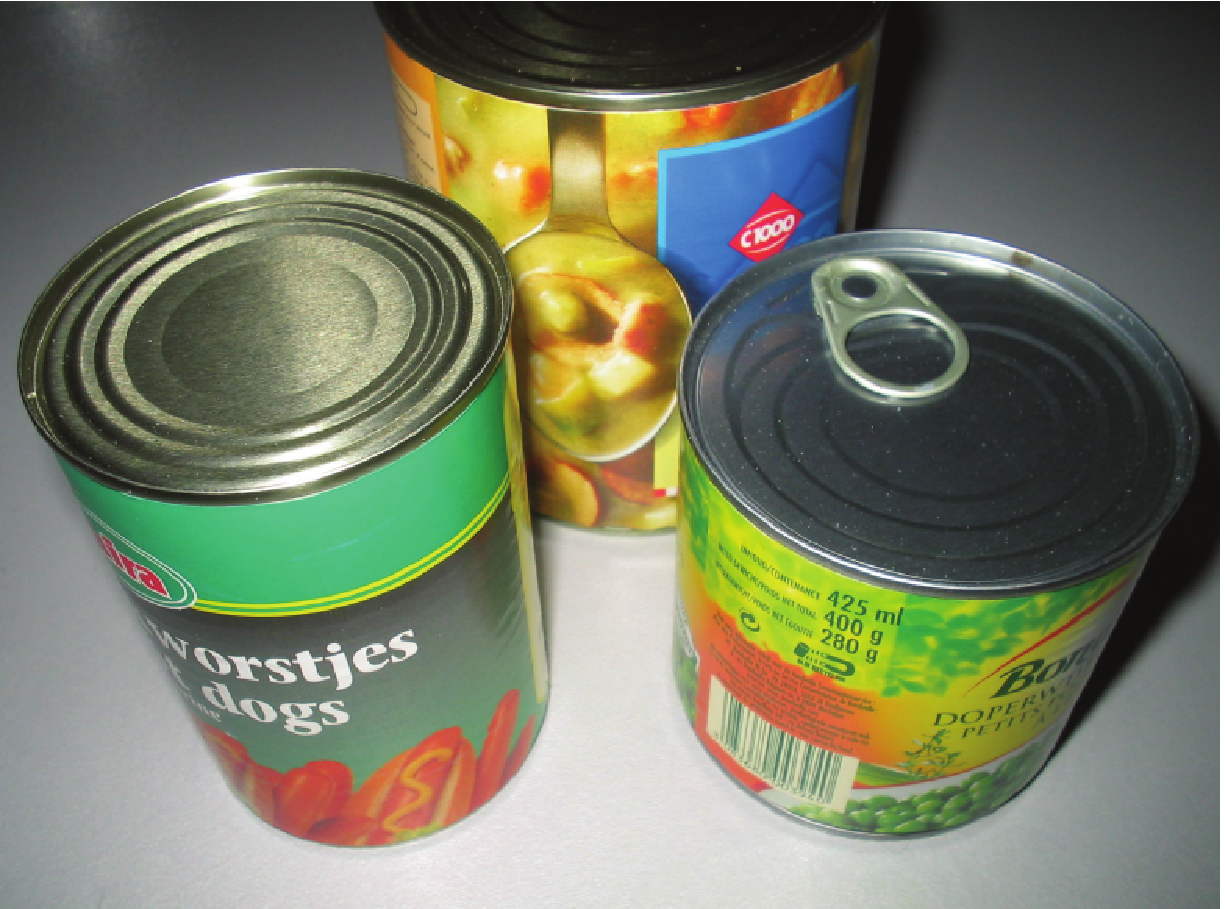
\includegraphics[width=6cm]{conserve.pdf} 
\end{wrapfigure}


Une boîte de conserve a souvent une forme de cylindre. Combien de face est-ce qu'une telle boîte possède ?

\begin{enumerate}
    \item
        Si on décolle l'étiquette, quelle forme a-t-elle ?
    \item

 Si on ouvre une boîte de conserve des deux côtés et qu'on la déplie, on obtient le patron d'un cylindre de révolution. À main levée, tracer un tel patron.
 \item
    Déterminer le périmètre de la base en fonction du rayon de cette base. En déduire la longueur de la face latérale. 
\item

    Réaliser le patron d'un cylindre de révolution de hauteur \SI{5}{\centi\meter} ayant pour base un disque de rayon \SI{3}{\centi\meter}. 

\end{enumerate}

De \cite{NRHooXFvgpp5}


%+++++++++++++++++++++++++++++++++++++++++++++++++++++++++++++++++++++++++++++++++++++++++++++++++++++++++++++++++++++++++++ 
\section{Cylindres de révolution}
%+++++++++++++++++++++++++++++++++++++++++++++++++++++++++++++++++++++++++++++++++++++++++++++++++++++++++++++++++++++++++++

\begin{definition}
Un cylindre de révolution est un solide engendré par la rotation d'un rectangle autour d'un de ses côtés.
\end{definition}

\begin{propriete}
   Les bases d'un cylindre de révolution sont deux disques identiques.
\end{propriete}


\begin{example}
    Dessiner un patron d'un cylindre de révolution de hauteur \SI{3}{\centi\meter} ayant pour base un disque de rayon \SI{1}{\centi\meter}.



    \begin{enumerate}
        \item
            On dessine une base, c'est à dire une disque de rayon \SI{1}{\centi\meter}.
\begin{center}
   \input{Fig_JHVRooIEVJMgooZERO.pstricks}
\end{center}
        \item


            La face latérale est un rectangle dont un côté est la hauteur du cylindre (\SI{3}{\centi\meter}) et l'autre est le périmètre du cercle (environ \SI{3.28}{\centi\meter})


\begin{center}
   \input{Fig_JHVRooIEVJMgooONE.pstricks}
\end{center}

        \item
            La seconde base se colle sur l'autre côté de longueur \SI{3.28}{\centi\meter} de la face latérale.
\begin{center}
   \input{Fig_JHVRooIEVJMgooTWO.pstricks}
\end{center}
    \end{enumerate}
\end{example}
